\documentclass[12pt,doublespacing,a4paper]{ouparticle}

%\usepackage[scaled]{helvet}
%\renewcommand\familydefault{\sfdefault} 
%\usepackage[T1]{fontenc}


\usepackage[authoryear]{natbib}
\usepackage{lineno}
\usepackage{pdfpages}
\usepackage{lscape}


\begin{document}

\title{An Evaluation of the Robustness of Length Based Indicators using Receiver Operating Characteristics.}

\author{%
\name{Laurence T. Kell}
\address{Centre for Environmental Policy, Imperial College London, London SW7 1NE}
\email{e-mail Lauriel@seapluslus.co.uk}
\and
\name{Co\'il\'in Minto}
\address{GMIT}
\email{Hans Gerritsen}
\address{Marine Institute}
}

\abstract{
%Scientific management advice for data rich stocks is based upon biological points and expert opinion to fix or meta-analyses to develop priors for difficult to estimate parameters. Whilst advice for data poor stocks is based upon life history parameters and outputs from data rich stock assessments to develop priors and propose indicators based upon life history traits.
%To help propose and develop robust and non-redundant productivity indicators the reliability and stability of the indices are evaluated with reference to the data rich set. 
}

\date{\today}

\keywords{}
 
\maketitle

\newpage


\linenumbers
\linespread{2}


\section{Introduction}

A substantial fraction of world fisheries are conducted on resources for which data are insufficient to conduct formal stock assessments and so status, productivity, and exploitation levels of many stocks and species are largely unknown \citep{thorson2015introduction}. Such stocks include by-caught, threatened, endangered, and protected species and are termed data-poor, data-limited, or information-poor. The adoption of the precautionary approach \citep[PA,][]{garcia1996precautionary}, however, still requires management plans and biological reference points for all stocks not just for the main commercial stocks where analytical assessments are available \citep{sainsbury2003ref}. 

Reference points are used in management plans as targets to maximise surplus production and as limits to minimise the risk of depleting a resource to a level where productivity is compromised. They must integrate dynamic processes such as growth, recruitment, mortality and connectivity into indices for exploitation level and spawning reproductive potential \citep{kell2015spawning}. In data poor situations life history parameters, such as maximum size and size at first maturity have been used as proxies for productivity \citep{roff1984evolution,jensen1996beverton,caddy1998short,reynolds2001life,denney2002life}. For example ICES uses indicators and proxy maximum sustainable yield (MSY) reference points based on length (e.g. the von Bertalanffy growth parameter $L_{\infty}$ and length at maturity $L_{mat}$) as part of a Precautionary Approach for stocks where only trends in mean length are available \citep[][]{ref}. 

An important characteristic of PA advice is that it should be robust to uncertainty. Where a robust control system is one that still functions correctly despite the presence of uncertainty \citep{radatz1990ieee, zhou1996robust}, while to be robust an indicator should be both reliable and stable. An indicator has high reliability if despite uncertainty it provides an accurate result, and it is stable if despite random error, similar results are produced across multiple trials. To evaluate the robustness of length based indicators and $MSY$ proxies  a simulation and sampling (i.e. sim-sam) procedure was employed where an Operatating Model (OM) was conditioned on life history parameters then psuedo data simulated using an Observation Error Model (OEM), allowing the indicators to be compared to the actual state of the resource.


\section{Material and Methods}

OMs were conditioned on life histories representing a range of population dynaics, namely turbot, brill, thornback ray, pollack and sprat. Scenarios that represent the main sources of uncertainty were also developed. Resource dynamics were simulated assuming an increasing trend in fishing mortality ($F$) that led to overfishing, then a recovery plan was implemented to bring fishing back to the $F_{MSY}$ level. Length based indicators were then generates using the OEM and compared to the fishing mortality in the OM, using Reciever Operating Characteristic (ROC) curves \citep{green1966signal}. A ROC curve can be thought of as a plot of the power as a function of the Type I Error of the decision rule. If the probability distributions for both detection and false alarm are known, the ROC curve is generated by plotting the cumulative distribution function (area under the probability distribution from  to the discrimination threshold) of the detection probability in the y-axis versus the cumulative distribution function of the false-alarm probability on the x-axis. A ROC analysis therefore provides a tool to select the best candidate indicators. 

\subsection{Methods}

For each species the life history parameters (\textbf{Table} \ref{tab:lh}) were used to parameterise a \cite{vonbert1957quantitative} growth curve, proportion mature-at-age, natural mortality \citep{lorenzen2002density} and a \cite{beverton1993dynamics} stock recruit relationship. Spawning stock biomass (SSB) was was used as a proxy for stock reproductive potential \citep[SRP][]{trippel_estimation_1999}. This assumes that fecundity is proportional to the mass-at-age of the sexually mature portion of the population irrespective of the demographic composition of adults \citep{murawski_impacts_2001} and that processes such as sexual maturity are simple functions of age \citep{matsuda_inconsistency_1996} and independent of gender.

These processes allow an equilibrium per-recruit model to be parameterised, which when combined with a stock recruitment relationship \cite{sissenwine1987alternative} is then used to condition a forward projection model to simulate the time series.

\subsubsection{Scenarios}

Even for data-rich stock assessments there is often large uncertainty about the dynamics \citep[i.e. model uncertainty;][]{punt2008refocusing}. This means that estimates of stock status are highly sensitive to assumptions about natural mortality-at-age \citep{jiao2012modelling}, vulnerability of age classes to the fisheries \citep{brooks2009analytical}, and the relationship between stock and recruitment which is difficult to estimate in practice \citep[e.g.][]{vert2013frequency,szuwalski2014examining,cury2014resolving,kell2015spawning,pepin2015reconsidering}. Therefore scenarios \citep[][]{ono2015importance,kell2015spawning,boorman1997recognising} representing these sources of uncertainty were developed for selection pattern, natural mortality, steepness of the stock recruitment relationship, recruitment variablility and sample size (\textbf{Table} \ref{tab:scen})

\begin{itemize}
 \item Selection pattern: \textbf{same as matirity ogive}; dome shaped; constant across all ages.
 \item Natural Mortality: \textbf{varies by age}; 0.2 
 \item Steepness of the stock recruitment: \textbf{0.7}; 0.9 
 \item Recruitment CV: \textbf{30\%}; \textbf{50\%}; \textbf{AR}
 \item Sample Size:\textbf{500}, \textbf{250}
\end{itemize}


\subsubsection{Indicators}


%\cite{punt2011among}


Simple catch rules have been developed for data poor stock, for example the “2 over 3” rule  of ICES (2012) which aims to keep stocks at their current level by multiplying recent catches by the trend in a biomass index. Catch rules that make use of more data sources have subsequently been developed (e.g. Fischer et al., submitted), using a rule of the form

\begin{equation} C_{y+1} = C_{y-1}rfb \end{equation}

The advised catch is based on the previous catch $C_{y-1}$, multiplied by three components $r$, $f$ and $b$, each representing a particular stock characteristic. Component $r$ corresponds to the trend in a biomass index, component $f$ uses a proxy  for the rateio $F:F_{MSY}$ based on length, and $b$ is a safeguard which protects the stock by not allowing catch to increase unlimitedly once the biomass index drops below a threshold. In this study we focus on the $f$ component, although the same approach can be used to screen any data source or even outputs from data rich assessments.

Empirical indicators based on length, used as proxies for exploitation rate, include

\begin{itemize}
 \item $L_{max5\%}$ mean length of largest 5\%
 \item  $L_{95\%}$ $95^{th}$ percentile
 \item  $P_{mega}$ Proportion of individuals above $L_{opt} + 10\%$
 \item  $L_{25\%}$ $25^{th}$ percentile of length distribution
 \item  $L_{c}$ Length at $50\%$ of modal abundance
 \item  $L_{mean}$ Mean length of individuals $> L_c$
 \item  $L_{max_{y}}$ Length class with maximum biomass in catch
 \item  $L_{mean}$ Meanlength of individuals $> L$
\end{itemize}

and potential reference points include

\begin{itemize}
 \item $L_{\infty}$
 \item $L_{mat}$
 \item $L_{opt} = L_{\infty}\frac{3}{3+\frac{M}{K}}$, assuming $M/K = 1.5$ gives $\frac{2}{3}L_{\infty}$
 \item $L_{F=M} =  0,75l_c+0.25l_{\infty}$
\end{itemize}


\subsubsection{Receiver Operating Characteristics}

Indicators and reference point may be biased and have poor precision due to uncertainty about life history parameters, lags between size distribution and exploitation levels, variability in recruitment and resonant cohort effects that can produce long term fluctuation in the time series \citep{botsford2014cohort,bjoernstad2004trends}. This means that the reference level that can best identify the system state is unlikely to be $L_{mean}/L_{F=M}$ but a multiple of it, i.e. the discrimination threshold. The discrimination threshold is the value of $L_{mean}/L_{F=M}$ at which the a stock is said to be undergoing overfishing. A ROC curve plots the true positive rate (TPR) against the false positive rate  (FPR) at various threshold settings. Risks are asymmetric, i.e. the risk of indicating overfishing is occurring when the stock is sustainably exploited is not the same as the risk of failing to identify overfishing, and so it may be desirable to adjust the threshold to increase or decrease the sensitivity to false positives.

The ROC curve is constructed by sorting the observed outcomes from the OM by their predicted scores (from the OEM) with the highest scores first. The cumulative True Positive Rate (TPR) and True Negative Rate (TNR) are then calculated for the ordered observed outcomes. The ROC curve can also be thought of as a plot of the power as a function of the Type I Error of the decision rule. If the probability distributions for both detection and false alarm are known, the ROC curve can be generated by plotting the cumulative distribution function (area under the probability distribution from  to the discrimination threshold) of the detection probability in the y-axis versus the cumulative distribution function of the false-alarm probability on the x-axis. A ROC analysis therefore provides a tool to select the best candidate indicators. 


\section{Results}


\textbf{Figure} \ref{fig:cor} Life history parameters

\textbf{Figure} \ref{fig:oms} shows the simulated exploitation history relative to $MSY$ reference points for each of the stocks for the base case. Fishing was initially low then increased to twice $F_{MSY}$, following which a recovery plan was implemented in order to reduce F to $F_{MSY}$. The coloured regions indicate exploitation levels.

\textbf{Figure} \ref{fig:samples} Example simulated length samples 

\textbf{Figure} \ref{fig:indicators} indicators 

\textbf{Figure} \ref{fig:roc} ROC curves

\textbf{Figure} \ref{fig:discrim} discrimination thresholds for each indicator. 



\section{Discussion}


\begin{description}
 \item[Uncertainty]  
 \item[Risk]     
 \item[Management Frameworks] 
 \item[Robustness]
 \item[Lessons for data poor case studies]  
 \item[Lessons for data rich case studies] 
\end{description}

%For risks to be managed in a consistent way given the range of uncertainties across data rich and poor stocks requires OMs to be condition on appropriate processes. This allows an evaluation of the relative value-of-information and the value-of-control. In the former case this involves demonstrating the benefit of obtain better knowledge and data, i.e. to move a stock between categories, and in the later to consider alternative forms of indicators and control rules to develop robust advice. ROC curves are related in a direct and natural way to a cost/benefit analysis of diagnostic decision making, i.e. can be used to identify the value of control

%Setting of appropriate reference levels in the f and b component of the rules, and the extent to which this could be done with tuning that depends on life-history traits and/or the nature of the time-series was addressed using tools developed under the MyDas project. The aim of MyDas is to develop and test a range of assessment models and methods to establish Maximum Sustainable Yield (MSY), or proxy MSY reference points across the spectrum of data-limited stocks. To tune a catch rule of the form r f b, requires selecting indicators and reference points for each of the r and b components and then finding multipliers and thresholds for the component in order to combine them into a single rule. Doing this on a stock specific basis can take considerable time using MSE alone, especially as a variety of indicators and reference points can be used.  Therefore an example was developed using a Receiver Operating Characteristic or ROC curve, to show how potential indicators and reference points can be screened for a range of uncertainties before conducting MSE. 


\section{Conclusions}

\begin{itemize}
 \item 
 \item 
 \item 
 \item 
\end{itemize}

\section{Acknowledgement}

Laurence Kell's involvement was funded through the MyDas project under the Marine Biodiversity Scheme which is financed by the Irish government and the European Maritime and Fisheries Fund (EMFF) as part of the EMFF Operational Programme for 2014-2020. 

\clearpage
\bibliography{/home/laurence/Desktop/refs.bib}
\bibliographystyle{apalike}


\clearpage
\section{Figures}

\newpage
\begin{figure}[h]
\centering
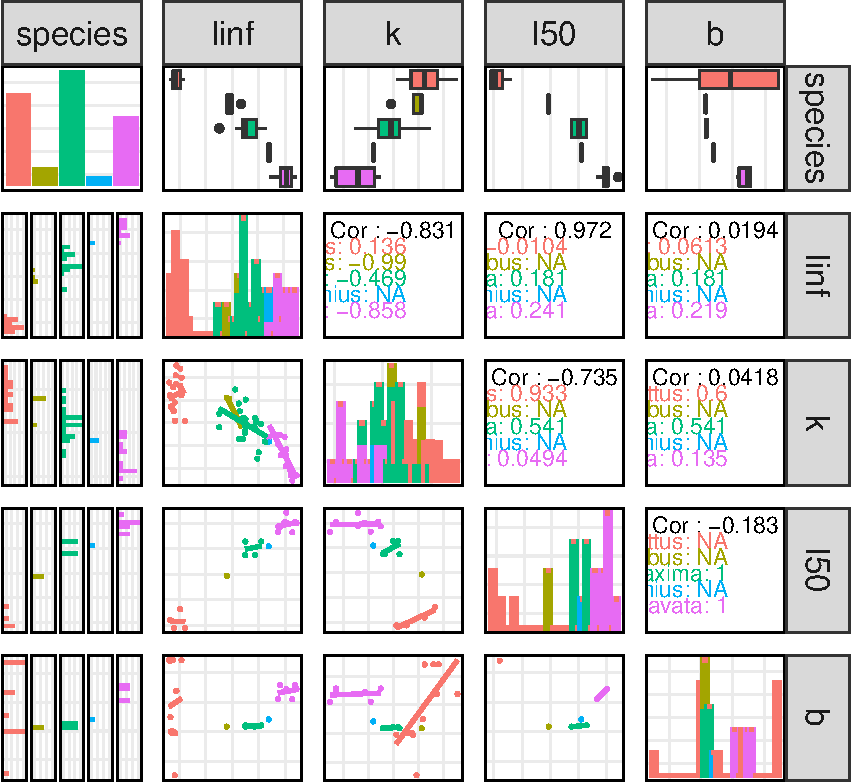
\includepdf[pages=1,pagecommand={},width=\textwidth]{roc-cor-1.pdf}
%\includegraphics[width=\textwidth]{om.png}
\caption{Life history parameters.}
\label{fig:cor}
\end{figure}

\newpage
\begin{figure}[h]
\centering
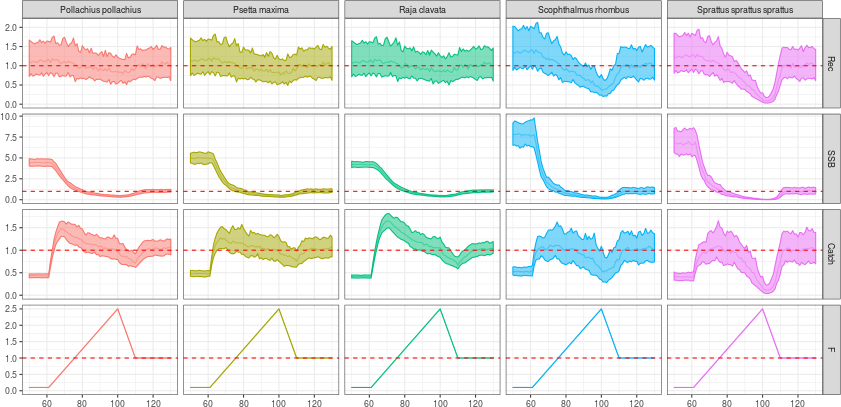
\includepdf[pages=1,pagecommand={},width=\textwidth]{roc-ts-1.pdf}
%\includegraphics[width=\textwidth]{lensamples.png}
\caption{Operating Models, showing exploitation history relative to $MSY$ reference points; fishing was initially low then increased to twice $F_{MSY}$ following which a recovery plan was implemented in order to reduce $F$ to $F_{MSY}$.}
\label{fig:oms}
\end{figure}

% js!K*o8%Lo$n


\newpage
\begin{figure}[h]
\centering
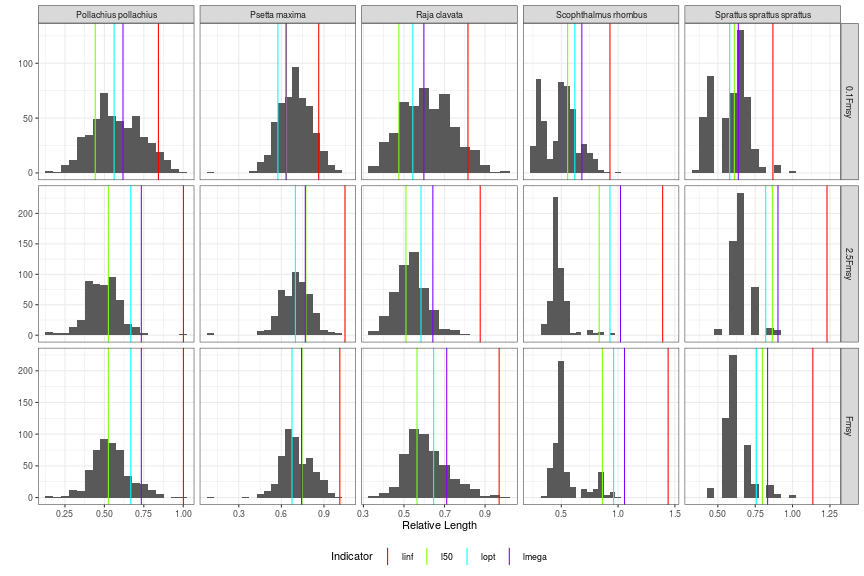
\includegraphics[width=\textwidth]{roc-lf-1.png}
\caption{Simulated length samples.}
\label{fig:samples}
\end{figure}

\newpage
\begin{figure}[h]
\centering
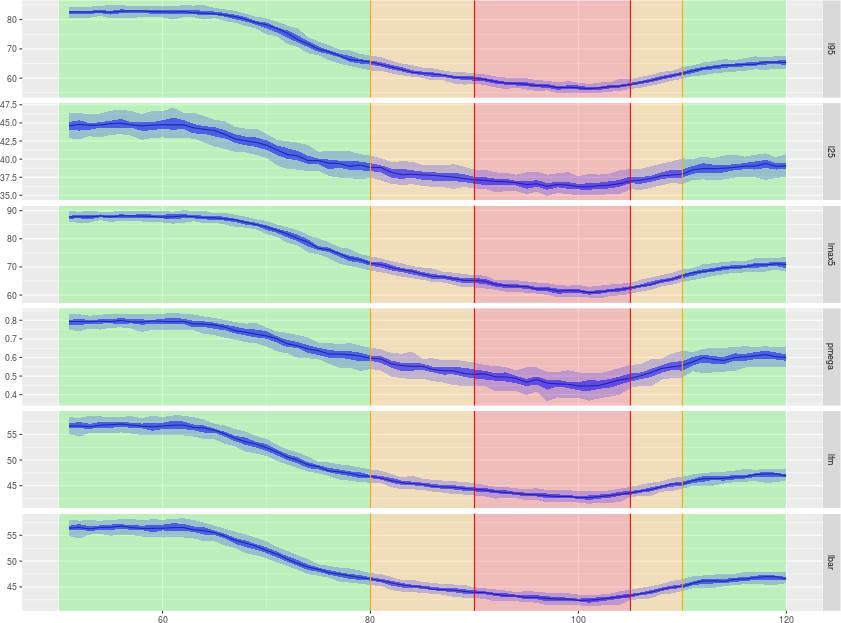
\includepdf[pages=1,pagecommand={},width=\textwidth]{roc-inds-1.png}
%\includegraphics[width=\textwidth]{indicatorTab.png}
\caption{Examples of indicators for the turbot base case; the coloured regions indicate exploitation levels relative to $F_{MSY}$, $F<F_{MSY}$ (green),  $F_{MSY} <F< 1.5F_{MSY}$ (yellow), and $F \geq 1.5F_{MSY}$ (red).}
\label{fig:indicators}
\end{figure}


\newpage
\begin{figure}[h]
\centering
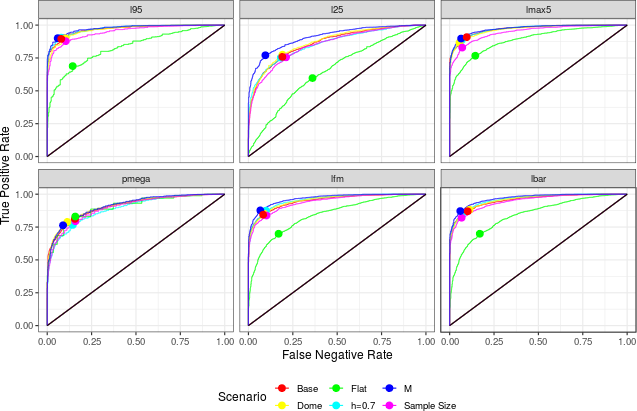
\includegraphics[width=\textwidth]{roc-overfish-roc-pollack-1.png}
\caption{Receiver Operating Characteristic curves.}
\label{fig:roc}
\end{figure}


\newpage
\begin{figure}[h]
\centering
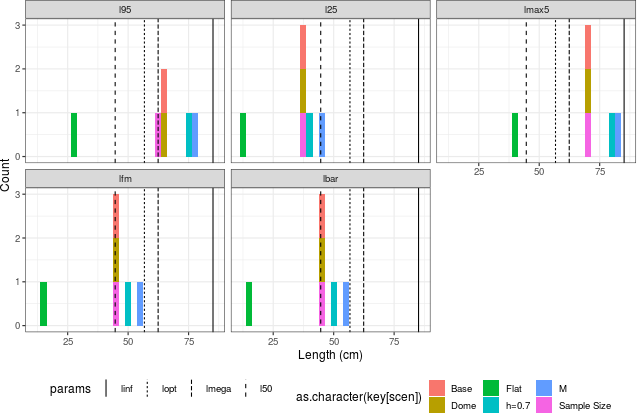
\includegraphics[width=\textwidth]{roc-overfish-ref-pollack-1.png}
\caption{Descrimnation thresholds.}
\label{fig:discrim}
\end{figure}

\clearpage
\section{Appendix}


2012a. ICES Implementation of Advice for Data-limited Stocks in 2012 in its 2012 Advice. ICES CM 2012/ACOM 68: 42 pp.

ICES. 2017a. Report of the ICES Workshop on the Development of Quantitative Assessment Methodologies based on Life-history traits, exploitation characteristics, and other relevant parameters for data-limited stocks in categories 3-6 (WKLIFE VI), 3-7 October 2016, Lisb. ICES CM 2016/ACOM:59: 106 pp.


\end{document}


